\documentclass[12pt,letterpaper]{report}
\usepackage{natbib}
\usepackage{geometry}
\usepackage{fancyhdr}
\usepackage{afterpage}
\usepackage{graphicx}
\usepackage{amsmath,amssymb,amsbsy}
\usepackage{dcolumn,array}
\usepackage{tocloft}
\usepackage{asudis}
\usepackage{booktabs}
\usepackage{rotating}
\usepackage{adjustbox}
\usepackage[pageanchor=true,plainpages=false,pdfpagelabels,bookmarks,bookmarksnumbered]{hyperref}

\begin{document}
%-----------------------front matter
\pagenumbering{roman}
\title{Fostering Collaborative Solutions in the Opioid Overdose Crisis: Law Enforcement as a Potential Partner in Reducing Fatalities}
\author{Seth Watts}
\degreeName{Doctor of Philosophy}
\paperType{Dissertation}
\defensemonth{October}
\defenseyear{2024}
\gradmonth{December}
\gradyear{2024}
\chair{Michael D. White}
\memberOne{Jacob T.N. Young}
\memberTwo{Alyssa W. Chamberlain}
\memberThree{Brandon del Pozo}
\memberFour{ }

\maketitle
\doublespace
\include{abstract}
\dedicationpage{}
\include{ack}
\tableofcontents
% This puts the word "Page" right justified above everything else.
\addtocontents{toc}{~\hfill Page\par}
% Asking LaTeX for a new page here guarantees that the LOF is on a separate page
% after the TOC ends.
\newpage
% Making the LOT and LOF "parts" rather than chapters gets them indented at
% level -1 according to the chart: top of page 4 of the document at
% ftp://tug.ctan.org/pub/tex-archive/macros/latex/contrib/tocloft/tocloft.pdf
\addcontentsline{toc}{part}{LIST OF TABLES}
\renewcommand{\cftlabel}{Table}
\listoftables
% This gets the headers for the LOT right on the first page.  Subsequent pages
% are handled by the fancyhdr code in the asudis.sty file.
\addtocontents{lot}{Table~\hfill Page \par}
\newpage
\addcontentsline{toc}{part}{LIST OF FIGURES}
\addtocontents{toc}{CHAPTER \par}
\renewcommand{\cftlabel}{Figure}
% This gets the headers for the LOF right on the first page.  Subsequent pages
% are handled by the fancyhdr code in the asudis.sty file.
\addtocontents{lof}{Figure~\hfill Page \par}
\listoffigures
%-----------------------body
\doublespace
\pagenumbering{arabic}
\include{chapter1}
\chapter{Study 1}

\chapter{Study 2}

\section{Introduction}

The opioid overdose crisis, one of the longest ongoing public health crises, worsened in recent years when opioid overdose fatalities eclipsed 80,000 (Center for Disease Control and Prevention [CDC], 2023). The crisis can be traced back to the 1990s and since then a host of policy changes and programs have been implemented to reduce opioid overdose fatalities. One of the most common state-level policy changes of the last couple decades has been the implementation of Naloxone Access Laws (NALs). According to the Legislative Analysis and Public Policy Association (LAPPA), every state has some form of a NAL, although the components of the policy varies (LAPPA, 2022). Additionally, Good Samaritan Laws (GSLs) have been signed into law in 50 states (and D.C.) which generally provide immunity to those who overdose as well as those who aid in helping the individual who overdosed, although the language varies from state to state (West \& Varacallo, 2023). With the expansion of naloxone accessibility and its ability to reverse opioid overdoses police departments have been increasingly outfitting their officers with naloxone (Lurigio et al., 2018). In addition to carrying naloxone, police departments have been involved in collaborative efforts with social outreach organizations to reduce opioid overdose fatalities (Donnelly et al., 2022; Formica et al., 2021; Yatsco et al., 2020). Both outfitting officers with naloxone and collaborative approaches have been found to be effective at reducing fatal opioid overdoses (Donnelly et al., 2022; Rando et al., 2015) although the empirical base is limited given this is a relatively new approach.

However, some research has found that officers develop negative attitudes towards people who use drugs (PWUDs), people who use opioids (PWUOs), naloxone, and drug treatment modalities as they respond to overdoses over time (Carroll et al., 2020; Murphy \& Russell, 2020, 2021). This has been described as a potential compassion fatigue effect, where officers lose empathy \& develop negative attitudes following repeatedly seeing traumatic incidents (Figley, 1995, 2002). Compassion fatigue is not confined to police work. Compassion fatigue has been highlighted across professional contexts (R. E. Adams et al., 2006). Within the police context, the development of negative attitudes over time has implications for their involvement in overdoses. Primarily, if officers develop negative attitudes over time their support for treatment may subside and there is the potential that it produces more punitive responses, which could hinder any collaborative or public health focused approach towards drug use (see Winstanley, 2020).

In this study we explore Tempe police officers’ perceptions and attitudes regarding naloxone, PWUDs/PWUOs, and their role in responding to opioid overdoses across multiple waves of surveys. We then investigate the compassion fatigue hypothesis to better understand officers’ attitudes and perceptions conditional on their frequency of responding to overdoses. The findings have implications for police involvement in opioid overdose response and police training focused on naloxone, substance use, and PWUOs. 

\section{Literature Review}
\subsection{Police attitudes towards naloxone and PWUDs}
The police have increasingly become involved in responding to opioid overdoses and administering naloxone to combat rising opioid overdose fatalities. In some cases, the police are involved in referral or diversion programs to meet opioid overdose survivors with the potential to engage with social services. Due to law enforcement frequently being the first point of contact for someone who overdoses and a shift towards a public health model in some localities (Beletsky et al., 2011; Silverman et al., 2012), there is the potential for police officers to act as a conduit to services. While officer attitudes towards these issues were unexplored previously, their increased role in the opioid overdose crisis has prompted research into this area. Recent literature has explored officer attitudes. This work primarily focuses on perceptions and attitudes towards substance use, naloxone, PWUDs/PWUOs, and their role in responding to opioid overdoses.

Prior work has found that officers have generally favorable attitudes towards naloxone and their role in responding to overdoses (Purviance et al., 2017; Wagner et al., 2016; White et al., 2021). Officers have reported feeling a sense of helplessness on scene at an overdose without being equipped with naloxone (Banta-Green et al., 2013; White et al., 2021). One way to improve officers’ ability to help effectively handle an overdose situation is to provide them with naloxone. In 2013, Deputy Director of the U.S. National Drug Control Policy emphasized the importance of law enforcement to carry naloxone (Michael Botticelli, 2013). Additionally, The Bureau of Justice Assistance highlighted that in addition to the ability to save lives, naloxone provides an improvement to job satisfaction among police officers (Bureau of Justice Assistance, n.d.). Officers within the Tempe Police Department were more likely to agree that they were glad to be carrying naloxone 10 months into the program compared with pre-intervention attitudes (White et al. 2021). Indeed, outfitting officers with a medication that reverses the effects of an overdose is generally viewed favorably among officers. Other research has noted that the police want to be able to effectively provide life-saving care to reverse the effects of an overdose indicating their desire to carrying naloxone (Purviance et al., 2017). And the idea of collaboration with public health agencies to address drug use is viewed as a more effective approach than traditional methods in some jurisdictions (Lloyd et al., 2023). 

Police officers also feel competent and confident when it comes to carrying and administering naloxone. Officers can effectively administer naloxone and are receptive to training (Lloyd et al., 2023; Pourtaher et al., 2022; Purviance et al., 2017; Wagner et al., 2016). Trainings developed to improve competency and confidence in administering naloxone have been successful in improving competency and confidence in handling overdose situations among police officers. Additionally, trainings have been implemented to combat opioid exposure myths among police officers and have been successful (del Pozo et al., 2021). 

However, other research has casted doubt on the role of the police as a collaborative entity in combatting the opioid overdose crisis (see Carroll et al., 2023). Police officers are not immune from stigmatizing views of PWUDs. While officers may have generally positive views of naloxone and their role in the opioid overdose crisis, much like the general population, they still have negative perceptions towards PWUDs (Barry et al., 2014; Calabrese \& Bell, 2019). For instance, studies have found that officers tend to agree that those who overdose are to blame (Beletsky et al., 2005; Wagner et al., 2016), naloxone enables PWUDs to continue using (Banta-Green et al., 2013; Burris et al., 2009), and that naloxone encourages risker drug use (Saunders et al., 2019). Some of the negative perceptions of PWUDs can be corrected through training (Winograd et al., 2019). However, others have shown that attitudes towards PWUDs may be less amenable following training modules (see Wagner et al., 2016). Additionally, Law enforcement involvement in overdose situations can lead to criminalizing PWUDs (Lowder et al., 2020; Van Der Meulen et al., 2021). The development of negative perceptions and/or attitudes towards PWUDs could influence their discretion at the scene of an overdose resulting in more punitive outcomes for PWUDs.

\subsection{Compassion fatigue}

In addition to general attitudes towards naloxone, PWUDs, and officers’ role in responding to opioid overdoses, research has found that with increased response to opioid overdoses, officers’ attitudes towards naloxone PWUDs decline. This is suggestive of a compassion fatigue effect. Compassion fatigue refers to the negative effect of vicarious traumatization. That is, an individual in an occupation where they care for and interact with individuals who experience traumatic events (e.g., first responders, therapists, etc.) may be vicariously traumatized and over time may become less empathetic and develop pessimistic attitudes (R. E. Adams et al., 2006; Figley, 1995). 

While qualitative has highlighted this potential compassion fatigue effect among police officers and other first-responders (Banta-Green et al., 2013; Saunders et al., 2019), more recent work has explored this finding quantitatively. Carroll et al. (2020) finds that as the frequency of overdose response increases, attitudes towards their scale of ‘enforcement overdose response efforts’ decline (0 to 15). Specifically, those who reported responding more than 4 times per month to an overdose has a composite score of 6.84. For those who had not responded to an overdose, their composite score was 8.13 which indicates a higher level of agreement towards law enforcement overdose response efforts. 

Likewise, Murphy and Russell (2020) investigate the compassion fatigue hypothesis using both bivariate and multivariate analyses for a sample of police officers in Pennsylvania. Murphy and Russell’s findings support the notion that officers feel trained and want to be involved in responding to opioid overdoses. However, they also find that officers have negative attitudes towards drug treatment and PWUDs and that these negative attitudes are related to frequency of overdose response and naloxone administrations (also see Murphy and Russell, 2021).

\section{Current Study}

I am interested in examining how officers’ attitudes have changed towards naloxone, their role in responding to opioid overdoses, and PWUDs over four waves of surveys. This broad interest is driven by the compassion fatigue literature that suggests officer attitudes may become more pessimistic, less empathetic, and less supportive of overdose response efforts as they respond to more opioid overdoses (cites). To evaluate the compassion fatigue hypothesis, I have two research questions:

1) Are officers’ attitudes towards naloxone, their role in responding to opioid overdoses, and their perceptions of PWUOs changing over time? 

\newtheorem{hypothesis}{Hypothesis}

\begin{hypothesis} Officer's attitudes towards naloxone, PWUOs, and their role in responding to opioid overdoses will change over time.\end{hypothesis}

2) Is opioid overdose response frequency associated with officer attitudes? 

\begin{hypothesis} Officer's attitudes towards naloxone, PWUOs, and their role in responding to opioid overdoses will have a relationship with opioid overdose response frequency. \end{hypothesis}

To answer these research questions, I use survey data that captures Tempe officers’ attitudes at different time points over a four-year period. To examine attitudinal change over time, I will employ unconditional linear growth models. To answer the second research question, I run pooled OLS regression models with wave fixed effects to explore how the frequency of opioid overdose response impacts officers’ attitudes.

\section{Methods}
\subsection{Setting}

Since 2020 the Tempe Police Department (TPD) has been involved in a collaborative effort with a social services organization – EMPACT – to reduce opioid overdose fatalities in Tempe, Arizona. This project, called the Tempe First-Responder Opioid Recovery Project, is funded by the Substance Abuse and Mental Health Services Administration (SAMHSA). The project trained and outfitted Tempe officers with naloxone in January of 2020 and created a 24/7 crisis hotline which officers contacted following an overdose incident to get in contact with a peer navigator (e.g., social outreach worker). Within days of the incident the peer navigator meets with the overdose survivor and their family/friends to provide information regarding potentially useful services (e.g., counseling, drug rehabilitation, housing information, transportation, etc.). Tempe officers have responded to more than 300 overdose incidents during the project. They have administered naloxone over 250 times in which it aided in a successful reversal of opioid overdose symptoms, and they have contacted the 24/7 crisis hotline approximately the same number of times. 

\subsection{Data}

The data for this study come from multiple waves of surveys administered throughout the duration of the Tempe ORP. The first wave of surveys was administered prior to the project in December of 2019 (n = 242). In October of 2020, the second wave of surveys was administered (n = 117). These two waves were the focus of our prior study looking at officers’ perceptions (White et al., 2021). The third wave was conducted in November of 2021 (n = 62) and the final wave was administered in March and April of 2023 (n = 109). The first three waves of surveys were administered electronically through Google Forms. Due to the decline in the response rate in wave 3, hard copy surveys were used for the fourth wave to improve our response rate.  I attended 10 patrol briefings with the project manager at TPD and handed out hard copy surveys to a total of 18 squads (111 officers). All four waves of surveys were voluntary and anonymous. The survey took approximately 12 to 15 minutes both electronically and hard copy. The surveys mostly comprised of true/false and Likert scale statements. Additionally, all four surveys utilize the OOKS and OOAS scales (Williams et al., 2013) and the NaRRC-B scale (Winograd et al., 2019). The survey also captured officer demographics.

\subsection{Dependent Variables}

I focus on three mean index measures: The role of the police, stigma towards PWUOs, and naloxone related beliefs. 

The role of the police is capturing by indexing four items, "I am glad to be carrying naloxone," "Tempe police officers should carry naloxone," "I feel better able to do my job carrying naloxone," and "Police should not respond to overdoses."\footnote{Police should not respond to overdoses is reverse coded.} The items produce a Cronbach's alpha that is above the conventional .70 threshold (\(\alpha = .774\)).

To measure stigma towards PWUOs I index four items, "People who overdose need to learn a lesson," "People who overdose deserve life-threatening outcomes," "People who overdose are to blame," and "Overdose survivors should be arrested."\footnote{There is an argument to be made that this item captures officer's perception of how they should handle overdose incidents. In terms of an improved Cronbach's alpha, it does not add any value in the Police Role measure. It does, however, improve the Stigma Towards PWUOs measure.} The items produce a Cronbach's alpha that is just below the conventional threshold of .70 (\(\alpha = .692\)).

Lastly, naloxone related beliefs is captured with five items, "People will use more if they have access to naloxone," "Users will be less likely to go to treatment due to naloxone," "Limit the number of naloxone administrations per person," "Naloxone enables PWUDs to continue their use," and "Providing naloxone means I condone opioid use." These items produce a Cronbach's alpha that is above the conventional .70 threshold (\(\alpha = .868\)).

The reasons these measures are chosen as outcome variables are two-fold. First, these items measure the concepts of interest and are of particular importance if they do indeed change over time or are influenced by opioid overdose response frequency. Theoretically, compassion fatigue would impact officer's attitudes towards these items. For instance, a decline in empathy towards PWUOs may produce pessimistic attitudes towards this population. It's possible that administering naloxone becomes associated with negative attitudes towards the medication if officers are encountering repeat overdose victims (cites). Secondly, prior work on this topic has used similar measures. Murphy and Russell (2020) use a few different items. To capture officer attitudes towards naloxone they provide the following statements in their survey instrument: “Increasing access and utilization of Narcan is a good solution to the opioid problem,” “Increasing access and utilization of Narcan provides individuals with a substance use disorder an excuse to continue their drug use,” “There should be a limit on how often someone who overdoses be administered Narcan.” While Carroll et al. (2020) use create a “OD response efforts scale” that contains five Likert scale items. Following their work, I use similar outcome variables that may be influenced by compassion fatigue. 

\subsection{Independent Variable}

There are two primary independent variables in this study. For the first research question, the wave of the survey is the independent variable of interest (i.e., 1, 2, 3, 4). For the second research question, opioid overdose response frequency is the independent variable of interest. This variable is measured on a five-point scale: “Never (0),” “Rarely (less than once per week) (1),” “Once per week (2),” “Once per shift (3),” and “Multiple times per shift (4).”

Control variables include whether the respondent is a patrol officer; reference category is non-patrol. Sex is measured as a dummy variable; males are the reference category. Race is captured as black, Hispanic, and other, while the reference category is white non-Hispanic. Education is measured as a dummy variable that indicates if the respondent has received a college education which includes two-year, four-year, and advanced degrees; the reference category includes high school diploma or a GED, and some college. Time spent at the Tempe Police Department is represented as a series of dummy variables 1-2 years, 3-5 years, 6-10 years, 11+ years at the department; the reference category is less than one year at the department. I then control for competence at the scene of an overdose. This variable is measured on a 4-point Likert scale from completely disagree (1) to completely agree (4). Specifically, this item states “I would be able to effectively deal with an overdose.” A dummy variable for having administered naloxone is included in the model as well. Lastly, I incorporate wave fixed effects to control for unobservable time invariant characteristics between the waves of the survey.

\subsection{Analytical Sample}
\subsection{Analytical Plan}

The analysis proceeds as follows. First, descriptive statistics of the sample will be presented. Second, to descriptively examine the change in attitudes over time, I will use three unconditional linear growth models. These will provide estimates for how attitudes have changed across the multiple waves of surveys over the course of the project. Lastly, to examine the relationship between opioid overdose response frequency and officer attitudes, I run three pooled OLS regression models with wave fixed effects.

\subsubsection{Uconditional Linear Growth Models}

\[Y_i = \beta_0 + \beta_1 Wave_i + \epsilon_i \]

Where \(Y_i\) is the outcome of interest (Police role, stigma towards PWUOs, and naloxone related beliefs) at wave \(i\). \(\beta_0\) is the intercept of outcome \(Y\). \(\beta_1\) is the coefficient for the primary independent variable -- waves of the survey. This represents the change in \(Y\) across the waves. Error is captured by \(\epsilon_i\).

\subsubsection{Pooled OLS Regression Models}

\[Y = \beta_0 + \beta_1 OD response frequency + \beta_n X_n + \alpha + \epsilon \]

Where \(Y\) is the outcome of interest (Police role, stigma towards PWUOs, and naloxone related beliefs). \(\beta_0\) is the intercept of outcome \(Y\). \(\beta_1\) is the coefficient for the primary independent variable -- opioid overdose response frequency. \(\beta_n X_n\) represents the coefficients for a vector of covariates described above. \(\alpha\) represents wave fixed effects to capture time invariant characteristics between the waves. Error is captured with \(\epsilon\).


\section{Results}
\section{Conclusion}



% descriptive stats
\begin{table}[htbp]\centering
\def\sym#1{\ifmmode^{#1}\else\(^{#1}\)\fi}
\caption{\centering Summary Statistics}
\begin{tabular}{l*{1}{cccc}}
\hline\hline
                &     Mean&       SD&      Min&      Max\\
\hline
Role of the police&     2.98&     0.63&     1.00&     4.00\\
Naloxone related beliefs&     2.21&     0.56&     1.00&     4.00\\
Stigma towards PWUOs&     2.38&     0.59&     1.00&     4.00\\
Never           &     0.15&     0.36&     0.00&     1.00\\
Rarely (less than once per week)&     0.45&     0.50&     0.00&     1.00\\
Once per week   &     0.32&     0.47&     0.00&     1.00\\
Once per shift  &     0.05&     0.22&     0.00&     1.00\\
Multiple times per shift&     0.02&     0.13&     0.00&     1.00\\
Ever administered naloxone&     0.25&     0.43&     0.00&     1.00\\
Patrol          &     0.57&     0.50&     0.00&     1.00\\
Female          &     0.16&     0.37&     0.00&     1.00\\
White           &     0.77&     0.42&     0.00&     1.00\\
Black           &     0.04&     0.19&     0.00&     1.00\\
Hispanic        &     0.14&     0.35&     0.00&     1.00\\
Other           &     0.05&     0.21&     0.00&     1.00\\
College degree  &     0.77&     0.42&     0.00&     1.00\\
Less than 1 year with&     0.05&     0.22&     0.00&     1.00\\
1-2 years with  &     0.07&     0.26&     0.00&     1.00\\
2-5 years with  &     0.15&     0.36&     0.00&     1.00\\
6-10 years with &     0.15&     0.36&     0.00&     1.00\\
11+ years with  &     0.58&     0.49&     0.00&     1.00\\
\hline\hline
\end{tabular}
\end{table}


% descriptive stats by wave
\begin{sidewaystable}[htbp]\centering
\def\sym#1{\ifmmode^{#1}\else\(^{#1}\)\fi}
\caption{\centering Summary Statistics by Wave}
\begin{tabular}{l*{4}{cccc}}
\hline\hline
                &   Wave 1&         &         &         &   Wave 2&         &         &         &   Wave 3&         &         &         &   Wave 4&         &         &         \\
                &     Mean&       SD&         &         &     Mean&       SD&         &         &     Mean&       SD&         &         &     Mean&       SD&         &         \\
\hline
Role of the police&     2.87&     0.63&         &         &     2.97&     0.57&         &         &     3.02&     0.74&         &         &     3.24&     0.53&         &         \\
Naloxone related beliefs&     2.18&     0.55&         &         &     2.23&     0.60&         &         &     2.21&     0.64&         &         &     2.23&     0.50&         &         \\
Stigma towards PWUOs&     2.30&     0.56&         &         &     2.39&     0.60&         &         &     2.55&     0.62&         &         &     2.45&     0.60&         &         \\
Never           &     0.19&     0.39&         &         &     0.17&     0.38&         &         &     0.13&     0.34&         &         &     0.07&     0.26&         &         \\
Rarely (less than once per week)&     0.47&     0.50&         &         &     0.43&     0.50&         &         &     0.40&     0.49&         &         &     0.47&     0.50&         &         \\
Once per week   &     0.29&     0.45&         &         &     0.32&     0.47&         &         &     0.39&     0.49&         &         &     0.37&     0.49&         &         \\
Once per shift  &     0.04&     0.19&         &         &     0.07&     0.25&         &         &     0.06&     0.25&         &         &     0.06&     0.23&         &         \\
Multiple times per shift&     0.01&     0.11&         &         &     0.02&     0.13&         &         &     0.02&     0.13&         &         &     0.03&     0.17&         &         \\
Ever administered naloxone&     0.02&     0.14&         &         &     0.22&     0.41&         &         &     0.45&     0.50&         &         &     0.67&     0.47&         &         \\
Patrol          &     0.47&     0.50&         &         &     0.53&     0.50&         &         &     0.53&     0.50&         &         &     0.85&     0.36&         &         \\
Female          &     0.16&     0.37&         &         &     0.14&     0.34&         &         &     0.18&     0.38&         &         &     0.19&     0.39&         &         \\
White           &     0.78&     0.41&         &         &     0.75&     0.44&         &         &     0.89&     0.31&         &         &     0.70&     0.46&         &         \\
Black           &     0.04&     0.19&         &         &     0.03&     0.17&         &         &     0.00&     0.00&         &         &     0.07&     0.26&         &         \\
Hispanic        &     0.13&     0.34&         &         &     0.17&     0.37&         &         &     0.07&     0.26&         &         &     0.18&     0.38&         &         \\
Other           &     0.05&     0.21&         &         &     0.06&     0.23&         &         &     0.04&     0.19&         &         &     0.05&     0.22&         &         \\
College degree  &     0.79&     0.41&         &         &     0.80&     0.40&         &         &     0.82&     0.38&         &         &     0.67&     0.47&         &         \\
Less than 1 year with&     0.04&     0.20&         &         &     0.01&     0.09&         &         &     0.00&     0.00&         &         &     0.14&     0.34&         &         \\
1-2 years with  &     0.07&     0.25&         &         &     0.04&     0.20&         &         &     0.03&     0.18&         &         &     0.14&     0.34&         &         \\
2-5 years with  &     0.17&     0.38&         &         &     0.13&     0.34&         &         &     0.03&     0.18&         &         &     0.20&     0.40&         &         \\
6-10 years with &     0.12&     0.32&         &         &     0.11&     0.32&         &         &     0.25&     0.44&         &         &     0.20&     0.40&         &         \\
11+ years with  &     0.60&     0.49&         &         &     0.70&     0.46&         &         &     0.68&     0.47&         &         &     0.32&     0.47&         &         \\
\hline\hline
\end{tabular}
\end{sidewaystable}


% growth model figure
\begin{figure}
    \centering
    \caption{\centering Unconditional Linear Growth Models}
    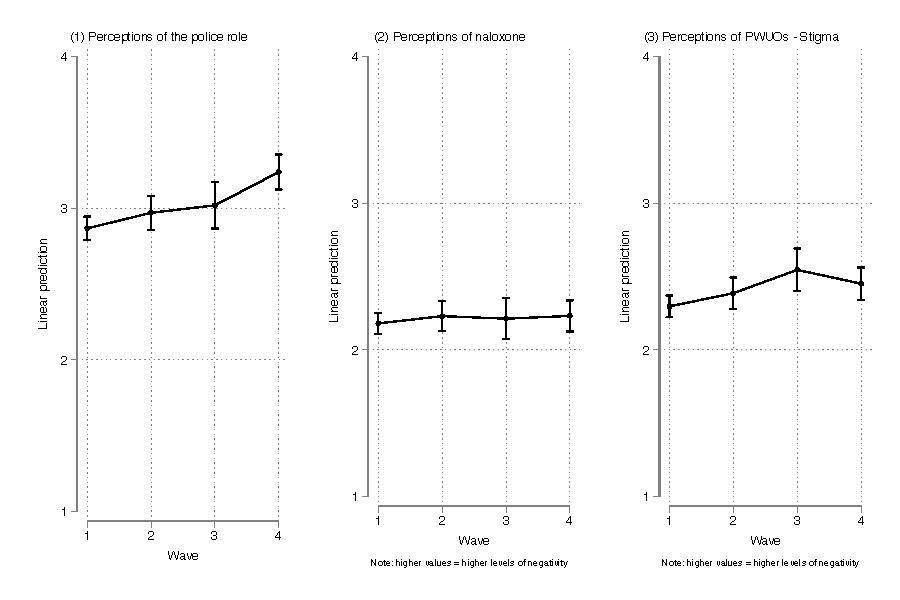
\includegraphics{figures/growth_models.pdf}
\end{figure}

% growth model coefficients table
\begin{table}[htbp]\centering
\def\sym#1{\ifmmode^{#1}\else\(^{#1}\)\fi}
\caption{\centering Unconditional Linear Growth Models}
\begin{tabular}{l*{3}{c}}
\toprule
                &\multicolumn{1}{c}{(1)}&\multicolumn{1}{c}{(2)}&\multicolumn{1}{c}{(3)}\\
                &\multicolumn{1}{c}{Role of the police}&\multicolumn{1}{c}{Naloxone related beliefs}&\multicolumn{1}{c}{Stigma towards PWUOs}\\
\midrule
Wave 2          &0.103 (0.069)         &0.050 (0.063)         &0.090 (0.066)         \\
\addlinespace
Wave 3          &0.152\sym{*} (0.087)         &0.032 (0.080)         &0.249\sym{***} (0.083)         \\
\addlinespace
Wave 4          &0.372\sym{***} (0.071)         &0.051 (0.065)         &0.155\sym{**} (0.067)         \\
\addlinespace
Constant        &2.867\sym{***} (0.040)         &2.181\sym{***} (0.036)         &2.297\sym{***} (0.038)         \\
\midrule
Observations    &      527         &      525         &      527         \\
\bottomrule
\multicolumn{4}{l}{\footnotesize Standard errors in parentheses}\\
\multicolumn{4}{l}{\footnotesize \sym{*} \(p<0.10\), \sym{**} \(p<0.05\), \sym{***} \(p<0.01\)}\\
\end{tabular}
\end{table}


% pooled reg models coefficients
\begin{table}[htbp]\centering
\def\sym#1{\ifmmode^{#1}\else\(^{#1}\)\fi}
\caption{\centering Pooled OLS Regression Models}
\begin{tabular}{l*{3}{c}}
\toprule
                &\multicolumn{1}{c}{(1)}&\multicolumn{1}{c}{(2)}&\multicolumn{1}{c}{(3)}\\
                &\multicolumn{1}{c}{Role of the police}&\multicolumn{1}{c}{Naloxone related beliefs}&\multicolumn{1}{c}{Stigma towards PWUOs}\\
\midrule
Rarely (less than once per week)&0.024 (0.082)         &-0.076 (0.076)         &-0.101 (0.078)         \\
Once per week   &0.000 (0.091)         &-0.005 (0.088)         &-0.069 (0.091)         \\
Once per shift  &0.034 (0.167)         &0.010 (0.133)         &-0.113 (0.138)         \\
Multiple times per shift&-0.246 (0.262)         &0.042 (0.206)         &-0.008 (0.213)         \\
Ever administered naloxone&0.190\sym{***} (0.068)         &-0.094 (0.076)         &-0.035 (0.078)         \\
Patrol          &-0.095 (0.066)         &0.081 (0.061)         &0.034 (0.063)         \\
Black           &0.220 (0.134)         &0.040 (0.134)         &-0.134 (0.139)         \\
Hispanic        &-0.001 (0.070)         &0.119 (0.073)         &-0.009 (0.075)         \\
Other           &-0.059 (0.119)         &0.096 (0.121)         &0.079 (0.125)         \\
Female          &0.070 (0.075)         &0.072 (0.069)         &-0.158\sym{**} (0.072)         \\
College degree  &-0.173\sym{***} (0.062)         &-0.054 (0.061)         &-0.030 (0.063)         \\
1-2 years with  &-0.137 (0.103)         &0.180 (0.145)         &-0.026 (0.150)         \\
2-5 years with  &-0.240\sym{**} (0.115)         &0.199 (0.133)         &0.001 (0.138)         \\
6-10 years with &-0.419\sym{***} (0.114)         &0.303\sym{**} (0.133)         &0.028 (0.138)         \\
11+ years with  &-0.318\sym{***} (0.096)         &0.114 (0.121)         &-0.040 (0.125)         \\
I would be able to effectively deal with an OD&0.172\sym{***} (0.053)         &-0.042 (0.040)         &0.099\sym{**} (0.041)         \\
Wave 2          &0.012 (0.071)         &0.037 (0.070)         &0.053 (0.072)         \\
Wave 3          &0.046 (0.110)         &0.042 (0.094)         &0.119 (0.098)         \\
Wave 4          &0.051 (0.092)         &0.067 (0.090)         &0.066 (0.093)         \\
Constant        &2.901\sym{***} (0.179)         &2.130\sym{***} (0.164)         &2.153\sym{***} (0.170)         \\
\midrule
Observations    &      459         &      458         &      459         \\
\(R^{2}\)       &    0.164         &    0.050         &    0.051         \\
\bottomrule
\multicolumn{4}{l}{\footnotesize Standard errors in parentheses}\\
\multicolumn{4}{l}{\footnotesize \sym{*} \(p<0.10\), \sym{**} \(p<0.05\), \sym{***} \(p<0.01\)}\\
\end{tabular}
\end{table}



\chapter{Study 3}
\chapter{Conclusion}
\include{chapter6}
%-----------------------back matter
{\singlespace
% Making the references a "part" rather than a chapter gets it indented at
% level -1 according to the chart: top of page 4 of the document at
% ftp://tug.ctan.org/pub/tex-archive/macros/latex/contrib/tocloft/tocloft.pdf
\addcontentsline{toc}{part}{REFERENCES}
\bibliographystyle{asudis}
\bibliography{dis}}
\renewcommand{\chaptername}{APPENDIX}
\addtocontents{toc}{APPENDIX \par}
\appendix
\include{appendix1}
\include{vita}
\end{document}
